A major challenge in transferring the knowledge from the source is to design a strategy to combine the source knowledge with the knowledge from the target task. In this section, we propose propose a combination strategy that using linear combination to combine the source and target knowledge. An important advantage of this strategy is that we can adjust the impact of the knowledge comes from the source model more flexibly by just modifying the value of its coefficient. As long as the source knowledge hurts the transfer model, we can reduce its impact to avoid negative transfer.

\hl{Intuitively}, when transferring the knowledge from another task, the performance of the model for the target task is greatly determined by the relationship of these two tasks. Here we use the $\mathcal{H}$-divergence to measure the relationship of two different tasks. $\mathcal{H}$-divergence can be defined as follow:
\begin{definition}
	(from Kifer et al. \cite{kifer2004detecting}) Given a domain $\mathcal{X}$ with two probability distributions, let $\mathcal{H}$ be a hypothesis class on $\mathcal{X}$ and denote by $I(h)$ the set for which $h \in \mathcal{H}$ is the characteristic function where $x\in I(h) \leftrightarrow h(x)=1$. The $\mathcal{H}$-divergence between these two probability distribution $D$ and $D'$ is 
	\begin{equation*}
	{d_{\mathcal{H}}}\left( {D,D'} \right) = 2\mathop {\sup }\limits_{h \in {\mathcal{H}}} \left| {{{\Pr }_D}\left[ {I(h)} \right] - {{\Pr }_{D'}}\left[ {I(h)} \right]} \right|
	\end{equation*}
\end{definition}
When $D$ and $D'$ are related, $d_{\mathcal{H}}\left( {D,D'} \right)$ is small and $d_{\mathcal{H}}\left( {D,D'} \right)$ is large when they are unrelated. Ben et al. \cite{ben2010theory} show that the performance of the target model is affected by the $\mathcal{H}$-divergence of the probability distributions of the two tasks. 

Then our single source self-defined category problem can be described as follow: Given a task  $T$ to distinguish whether an example is from one certain category $C$ from a domain $\mathcal{X} \times \mathcal{Y}$ with $D$ probability distribution over $\mathcal{X}$, $\mathcal{X}$ is the input feature and $\mathcal{Y}$ is the label set $\{1,-1\}$. We use an examples with label 1 to denote the positive example (i.e. belongs to the category) and an example with label -1 to denote the negative example (i.e. not belong to the category). We assume that we have another source model $f'$ trained from another independent task $S$ on another domain $\mathcal{X'} \times \mathcal{Y'}$ with $D'$ probability distribution over $\mathcal{X'}$ and $S$ and $T$ are related. We assume that a small training set $T_{train}=\{(x,y)\} \subset \mathcal{X}\times \mathcal{Y}$, $\mathcal{X}$ is given. We want to learn a classification problem $f: \mathcal{X} \rightarrow \mathcal{X}$ from $T_{train}$ incorporating with $f'$ so that $f$ can perform well on a independent testing set $T_{test}=\{(x,y)\} \subset \mathcal{X} \times \mathcal{Y}$.

Here, let's set the both source and target model $f$ and $f'$ in the hypothesis space of function $\mathcal{H}$ which equals to space of all the linear models of the form. 
\begin{equation}
f(x)=w^Tx+b
\end{equation}
%where $\phi(x)$ is a feature mapping that maps the input space into a another high or even possible infinite dimensional space.

To leverage the knowledge from the source model $f'$, we propose a method where a part of the decision of the target model $f$ comes from the decision of the source model $f'$. This process can be written as:
\begin{equation}\label{eq:single:linear}
\begin{aligned}
 f(x) = & w^T\phi(x)+b+\gamma f'(x) \\
\text{st.} \qquad & f'(x) = w'^T\phi(x)
\end{aligned}
\end{equation}

\begin{figure}
	\centering
	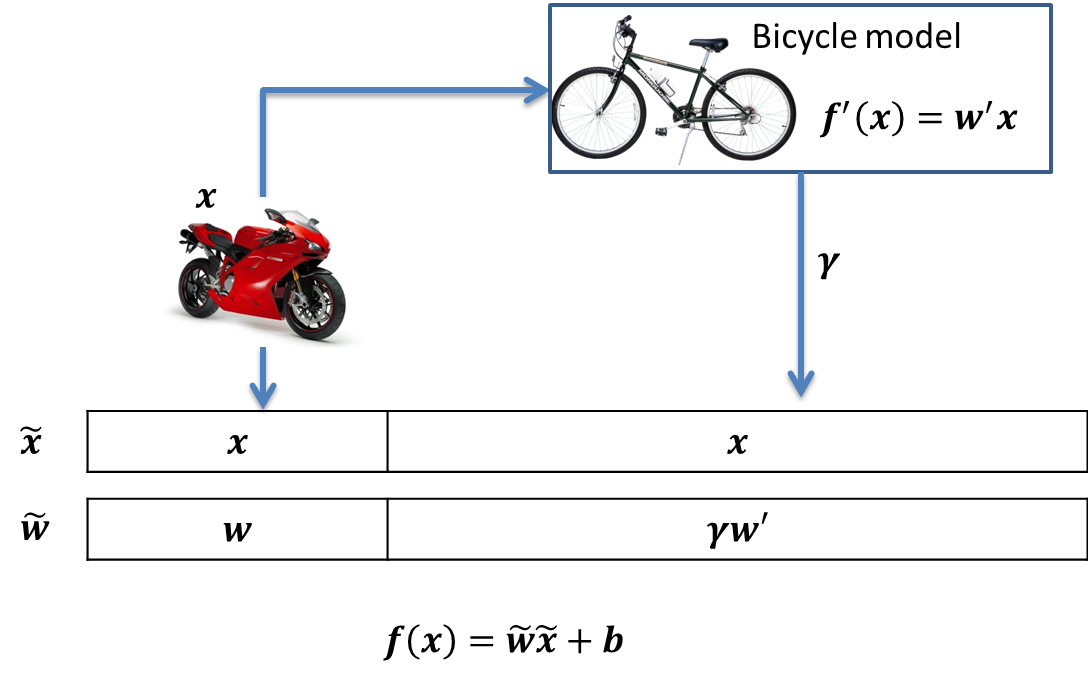
\includegraphics[scale=.6]{transfer/fig/argumentation.png}
	\caption{A graphical representation of linear combination. The score from the source model can be considered as an auxiliary feature and the transfer parameter controls the value of the auxiliary feature.}\label{fig:single:arg}
\end{figure}
Where $\gamma$ is called the transfer parameter $\gamma$ that controls the amount of the knowledge transferred from the source model $f'$. 
While combining the knowledge linearly, we can have several advantages especially when we use linear model such as SVM.

The first advantage is simplicity. Given a example $x$ and a source model $f'$, to consider the decision from the source model, we can simply add its score $f'(x)$ in to affect the decision of the target model. It is equivalent to the data argumentation approach where the score of the source model is used as the auxiliary feature (see Figure \ref{fig:single:arg}). Accordingly, the extra dimension which is set to 1, is added into the hyperplane $w$. By introducing the auxiliary information from the source model, we expect to reduce the bias from the target training set. As a result, we can successfully transfer a transfer learning problem into a traditional machine learning problem with data argumentation.  
Another advantage is flexibility. By using the transfer parameter to control the amount of the knowledge from the source model, the model for the target task is more adaptive to various of situation. Previous work  \cite{kuzborskij2013n} \cite{tommasi2014learning} just consider two situations: unrelated source and positive correlated source. Here we add another situation negative correlated source and expand the previous situation into 3:
\begin{itemize}
	\item When the two tasks are not related, it is expected to get a random score from the source model and the transfer parameter should be set to 0 to ignore it. Therefore, the target model won't affected by the noisy dimension and is less likely to suffer from negative transfer. In the extreme case where the transfer parameter is set 0, no auxiliary information is introduced to the target task and therefore, we can guarantee that, at least, negative transfer won't happen.
	\item When the source and target tasks are positive correlated, i.e. for a positive example $x_p$ and a negative example $x_n$, we have $f'(x_p)>f'(x_n)$, we expect the transfer parameter to be positive. Therefore, the positive and negative examples are more distinct and can be better distinguished by the hyperplane.
	\item  For the same reason above, we expect the transfer parameter to be negative if the two tasks are negative correlated.
\end{itemize}

Therefore, let $\tilde{x} = (x,x)$ and $\tilde{w} = (w,\gamma w')$.
With the LS-SVM setting, our transfer problem can be solved by solving the following optimization problem with argument data:
\begin{equation}\label{eq:single:reg}
	\begin{aligned}
	\min \qquad& L_{LSSVM}(\tilde{w}) = \frac{1}{2}{\left\| \tilde{w} \right\|^2} + \frac{C}{2}\sum\limits_{i = 1}^l {{e_i ^2}}\\
	\text{s.t.}\qquad& \tilde{w} = (w,\gamma w')\\
	&{y_i} = \tilde{w} {\tilde{x_i}} + b + {e _i} \quad   \text{for} \quad i \in \left\{ {1,2,...,l} \right\}\\
	\end{aligned}
\end{equation}
When we consider the transfer parameter $\gamma$ as a constant that can be determined by certain prior knowledge, to regularize  $\left\|\tilde{w}\right\|^2$ is equivalent to regularize $\left\|\tilde{w}-\gamma w'\right\|^2$. Therefore, function \eqref{eq:single:reg} can be represented as:
\begin{equation}\label{eq:single:formreg}
\begin{aligned}
\min \qquad& L_{\gamma}(w) = \frac{1}{2}{\left\| {w}-\gamma w' \right\|^2} + \frac{C}{2}\sum\limits_{i = 1}^l {{e_i ^2}}\\
\text{s.t.}\qquad& {y_i} = {w} {{x_i}} + b + {e _i} \quad   \text{for} \quad i \in \left\{ {1,2,...,l} \right\}\\
\end{aligned}
\end{equation}

To solve the problem \eqref{eq:single:formreg}, we first introduce some important notations used in the rest of this chapter in Table \ref{tab:single:notation}. We use any letter with apostrophe to denote the information from the source data, e.g. if $f(x)$ denotes the model for the target task, $f'(x)$ denotes the model for the source one.

% Table generated by Excel2LaTeX from sheet 'Sheet1'
\begin{table}
	\centering
	\caption{\hl{Notations used in this chapter}}
	\begin{tabular}{|c|L{14cm}|}
		\hline
		$f'(x)$ & binary model for source task \\
		\hline
		$f(x)$  & binary model for target task \\
		\hline
		$\phi(x)$ &  function mapping the input sample into a high dimensional feature space. \\ \hline
		%    $K(x,x)$ & kernel matrix with  $\phi(x_i) \cdot\phi(x_j)$ corresponding to its element $(i,j)$\\ \hline
		$X$     & instance matrix with each row representing one instance \\\hline
		$\boldsymbol{W} $    & (N+1)-column hyperplane matrix for target task. Each column represents one hyperplane of a binary model \\\hline
		$\boldsymbol{W'}$    & hyperplane matrix for the source task \\\hline
		$\boldsymbol{a'} $   & the Lagrangian multiplier matrix for source problem. Each column represents a set of Lagrangian multiplier for a binary SVM model \\\hline
		$\boldsymbol{a} $    & the Lagrangian multiplier matrix for target problem \\
		\hline
		$\boldsymbol{b'},\boldsymbol{b}$  & the bias vector for source and target task \\
		\hline
		$\boldsymbol{a_i}$ & $i_{th}$ column of matrix $\boldsymbol{a}$ \\ \hline
		%    $d_\gamma$ &  diagonal matrix with$\left[ {{\gamma _1},...,{\gamma _N}} \right]$ in its main diagonal\\\hline
		$\boldsymbol{\beta}$ & row vector $\left[ {{\beta _1},...,{\beta _N}} \right]$ to control the prior knowledge for the new category\\ \hline
		$\varepsilon_{ny_i}$&loss parameter. $\varepsilon _{n{y_i}}=1$ if $n=y_i$ and 0 otherwise\\ \hline
		$\psi$, $\psi^{-1}$ & $\psi$ is the modified kernel matrix for solving binary LS-SVM and $\psi^{-1}$ is the inverse matrix of $\psi$\\ \hline
	\end{tabular}%
	\label{tab:single:notation}%
\end{table}%

The primal Lagrangian for this optimization problem \ref{eq:single:formreg} given the unconstrained minimization problem can be written as: 
\begin{equation}
	{L_\gamma }\left( {w,b,\alpha ,e} \right) = \frac{1}{2}{\left\| {w - \gamma w'} \right\|^2} + \frac{C}{2}\sum\limits_{i = 1}^l {{e _i}^2}  - \sum\limits_{i = 1}^l {{\alpha _i}\left\{ {w{x_i} + b + {e_i} - {y_i}} \right\}} 
\end{equation}
The optimal solution can be found by satisfying the following condition:
\begin{eqnarray}\label{eq:single:lssvm-deriv}
\begin{aligned}
\frac{{\partial L}}{{\partial w}} = 0 &\to w = \gamma w' + \sum\limits_i^l {{\alpha _i}{x_i}} \\
\frac{{\partial L}}{{\partial b}} = 0 &\to \sum\limits_i^l {{\alpha _i} = 0} \\
\frac{{\partial L}}{{\partial e_i}} = 0 &\to C{e_i} = {\alpha _i} \qquad i = 1,...,l\\
\frac{{\partial L}}{{\partial {\alpha _i}}} = 0 &\to {y_i} = {w} {{x_i}} + b + {e _i}\qquad i = 1,...,l\\
\end{aligned}
\end{eqnarray}

Let $X=\left[x_1,x_2,...,x_l\right]$ and $Y=[y_1,y_2,...,y_l]$, Eq \eqref{eq:single:lssvm-deriv} can be written in the following compact format:

\begin{equation}\label{eq:single:matrixsolve}
	\left[\begin{array}{cccc}
	\mathbf{I}&0&0&-X^T\\
	0&0&0&-Y^T\\
	0&0&C\mathbf{I}&-I\\
	X&Y&I&0
	\end{array}\right]
	\left[\begin{array}{c}w-\gamma w'\\b\\e\\\alpha
	\end{array}\right]	= \left[\begin{array}{c}0\\0\\0\\\mathbf{1}
	\end{array}\right]
\end{equation} 
where $\mathbf{I}$ is an identity matrix and $\mathbf{1}$ is a column  vector whose elements are 1. 

In real applications, when we have $n$ single source categories and their corresponding source model $f'_1(x),f'_2(x),...,f_n(x)$, their loss function can be represented as:

\begin{equation}\label{eq:single:unionreg}
\begin{aligned}
\min \qquad& L_{\gamma}(w_1,w_2,...,w_n) = \frac{1}{2}\sum\limits_{i = 1}^n{\left\| {w_i}-\gamma_i w_i' \right\|^2} + \frac{C}{2}\sum\limits_{i = 1}^n\sum\limits_{j = 1}^l {{e_{ij} ^2}}\\
\text{s.t.}\qquad& {y_{ij}} = {w_i} {{x_i}} + b_i + {e _{ij}} \quad   \text{for} \quad i \in \left\{ {1,2,...,l}  \right\}, j \in {1,2,...,n}\\
\end{aligned}
\end{equation}
Let $\mathbf{W} = [w_1,w_2,...,w_n]$, $\mathbf{W'} = [w'_1,w'_2,...,w'_n]$ and $D(\gamma)$ be the diagonal matrix $diag(\gamma_1,\gamma_2,...,\gamma_n)$. The corresponding solution for problem \eqref{eq:single:unionreg} is:

\begin{equation}
\left[\begin{array}{cccc}
\mathbf{I}&0&0&-X^T\\
0&0&0&-Y^T\\
0&0&C\mathbf{I}&-I\\
X&Y&I&0
\end{array}\right]
\left[\begin{array}{c}\mathbf{W}- D(\mathbf{\gamma}) \mathbf{W'}\\b\\e\\\alpha
\end{array}\right]	= \left[\begin{array}{c}0\\0\\0\\\mathbf{1}
\end{array}\right]
\end{equation} 
 We can see that Eq. \eqref{eq:single:unionreg} can be solved by directly once the transfer parameters $\gamma=\{\gamma_i|i=1,...,n\}$ is determined.



